\documentclass{article}
\usepackage{url}
\usepackage{graphicx}
\usepackage{cellspace} 
\setlength{\cellspacetoplimit}{6pt}
\setlength{\cellspacebottomlimit}{6pt}

\newcommand{\toolname}{ROC Tool}
\newcommand{\toolnameIT}{\textit{ROC Tool}}
\newcommand{\toolnameITB}{\textit{ROC Tool}~}
\newcommand{\mainfilenameNO}{ROC\char`_Tool.R}
\newcommand{\mainfilename}{\texttt{\mainfilenameNO}}
\newcommand{\mainfilenameB}{\texttt{\mainfilenameNO}~}

\renewcommand*\contentsname{Content}

\title{\toolname: Compute ROC curves and iso-PM ROC Curves.}
\author{Lavazza Luigi, Morasca Sandro, and Rotoloni Gabriele}
\date{Version: 20250807}

\begin{document}
	
	\maketitle
	
	\toolnameITB is a tool that allows the user to visualize ROC curves and easily perform more advanced analysis on them. Specifically, the tool allows users to plot multiple ROC curves and their Regions of Interest, compute AUC and RRA, and plot multiple iso-PM curves.
	
	This documentation file can be accessed by pressing the "Help" button inside the application.
	
	For more information on how Regions of Interest, RRA, and iso-PM curves work, refer to the following paper: [XXXX]. If you use this tool for your research, please reference that paper.
	
	\newpage
	
	\tableofcontents
	
	\newpage
	
	\section{Installation and Execution}
	
	\subsection{Repository structure}
	\toolnameITB can be downloaded from GitHub (\url{kaal}). The repository contains the following files:
	\begin{itemize}
		\item \textbf{iRRA.zip} This is the R package needed to compute Regions of Interest (RoI) and RRA.The package was developed for the following paper~\ref{morasca2020assessment};
		\item \textbf{\mainfilenameNO} Is the R file containing the Shiny application.
		\item \textbf{utils} Contains all other R files needed to perform all computations needed for iso-PM curves.
		\item \textbf{doc} Contains this PDF file.
	\end{itemize}
	
	\subsection{Before running the tool}
	Before running the tool, it is necessary to install all needed packages.
	All packages except iRRA are automatically installed (if not already installed) when the tool is executed.
	
	iRRA has to be manually installed. In RStudio, the user needs to go to \texttt{Tools -> Install Packages...}. In the dialog window, select Package Archive File in the Install from: menu, and then select the \texttt{iRRA.zip} file. It is possible to verify if the installation went well by executing \texttt{library(iRRA)}.
	
	If the RStudio is not able to install iRRA this way, it is also possible to extract \texttt{iRRA.zip} and then move the extracted folder manually in the R folder that contains all the installed libraries (The user can see where the folder is with the \texttt{.libPaths()} function).
	
	\subsection{Execute the tool}
	To execute the tool the user needs to open the \mainfilenameB file and press the "Run App" button on the top-right corner of the source code pane.
	
	\section{Performance Metrics Supported by the Tool} \label{sec:pmSection}
	Given a confusion matrix like in Table~\ref{tab:confusionMatrix}, allows for the computation of multiple performance metrics (abbreviated in this document as PM). Table~\ref{tab:PMlist} indicates all the possible iso-PM ROC curves that can be computed with this version of the tool. 
	
	Note that, while in the original paper we refer to Matthews Correlation Coefficient as $\phi$, this tool uses the term MCC, which should be easier to recognize for people from different research fields.
	
	\begin{table}[h!]
		\label{tab:confusionMatrix}
		\centering
		\caption{Confusion Matrix.}
		\begin{tabular}{SlSlSlSl}
			\multicolumn{1}{l|}{}                             & \textbf{Actual Positives} & \multicolumn{1}{l|}{\textbf{Actual Negatives}} &               \\ \cline{1-3}
			\multicolumn{1}{l|}{\textbf{Estimated Positives}} & \multicolumn{1}{c}{TP}    & \multicolumn{1}{c|}{FP}                        & EP=TP+FP      \\
			\multicolumn{1}{l|}{\textbf{Estimated Negatives}} & \multicolumn{1}{c}{FN}    & \multicolumn{1}{c|}{TN}                        & EN=TN+FN      \\ \cline{1-3}
			& AP=TP+FN                  & AN=TN+FP                                       & n=AP+AN=EP+EN
		\end{tabular}
	\end{table}
	
	\begin{table}[h!]
		\label{tab:PMlist}
		\centering
		\caption{List of all PMs supported by the tool}
		\begin{tabular}{SlSlSlSl}
			\hline
			\textbf{Metric} & \textbf{Aliases}                      & \textbf{Formula} & \textbf{Values Range} \\ \hline
			TPR             & True Positive Rate, Recall            & $\frac{TP}{AP}$                & {[}0,1{]}             \\
			FPR             & False Positive Rate, Fallout          & $\frac{FP}{AN}$                 & {[}0,1{]}             \\
			MCC             & Matthews Correlation Coefficient, $\phi$ & $\frac{TP*TN-FP*FN}{\sqrt{EN*EP*AN*AP}}$                & {[}-1,1{]}            \\
			BA              & Balanced Accuracy                     & $\frac{TPR+TNR}{2}$                & {[}0,1{]}             \\
			Gmean           & -                                     & $\sqrt{TPR*TNR}$                & {[}0,1{]}             \\
			GM              & -                                     & $\frac{2*TPR*TNR}{TPR+TNR}$                & {[}0,1{]}             \\
			D2H             & Distance to Heaven (normalized)                   & $\sqrt{\frac{(1-TPR)^2+FPR^2}{2}}$                & {[}0,1{]}          \\
			precision       & PPV, Positive Precision Value         & $\frac{TP}{EP}$                 & {[}0,1{]}             \\
			F-score         & F1                                    & $\frac{2*precision*TPR}{precision+TPR}$                & {[}0,1{]}             \\
			NPV             & Negative Precision Value              & $\frac{TN}{EN}$                & {[}0,1{]}             \\
			TNR             & True Negative Rate, Specificity       & $\frac{TN}{AN}$                  & {[}0,1{]}             \\
			NM              & Negative F1, Negative F-Score         & $\frac{2*NPV*TNR}{NPV+TNR}$                 & {[}0,1{]}             \\
			Markedness      & -                                     & $precision - (1 - NPV)$                & {[}-1,1{]}            \\ \hline
		\end{tabular}
	\end{table}
	
	\subsection{Cost}
	This tool also allows to draw families of iso-cost curves. In this tool, "cost" is the misclassification cost, which is computed as
	
	\begin{equation} \label{eq:mccost}
		MC = cFP*FP + cFN*FN
	\end{equation}
	
	where FP and FN are False Positives and Negatives, respectively, and cFP and cFN are the relative cost for each misclassified element. This tool considers a normalized version of MC, as in Formula~\ref{eq:normCost}. 
	
	\begin{equation} \label{eq:normCost}
		NC = \lambda*\frac{1}{1+k}*(1-TPR) + (1-\lambda)*\frac{k}{1+k}*FPR
	\end{equation} 
	
	Where $\lambda = \frac{cFN}{cFN+cFP}$, and $k = \frac{AN}{AP}$. More details can be found in the following paper~\cite{morasca2020assessment}.
	
	\section{How to Use the Tool}
	Figure~\ref{fig:screen1} shows the tool when opened. On the top-left corner there are four buttons:
	\begin{itemize}
		\item \textbf{Menu} Allows player to add new curves, or modify curves that were already loaded in the tool. See Section~\ref{ssec:menus} for more details.
		\item \textbf{Open Configuration} Allows the user to open a project saved in a previous session. See Section~\ref{ssec:oploconfigs} for more details.
		\item \textbf{Reset} Clears the tool, allowing the user to start again. The tool will ask the user to press the "Reset" button again to confirm the choice.
		\item \textbf{Help} Pressing this button will open this PDF file.
	\end{itemize}
	
	\begin{figure}[h!]
		\centering
		\caption{First screen of the tool.}
		\label{fig:screen1}
		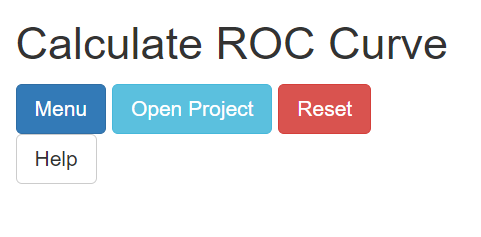
\includegraphics[width=1\linewidth]{Figures/screen1.png}
	\end{figure}
	 
	 \subsection{Using the Menu} \label{ssec:menus}
	 Figure~\ref{fig:screenMenu} shows the menu. In this menu the user can load a ROC curve and decide to generate different iso-PM curves.
	 
	 \begin{figure}[h!]
	 	\centering
	 	\caption{Menu.}
	 	\label{fig:screenMenu}
	 	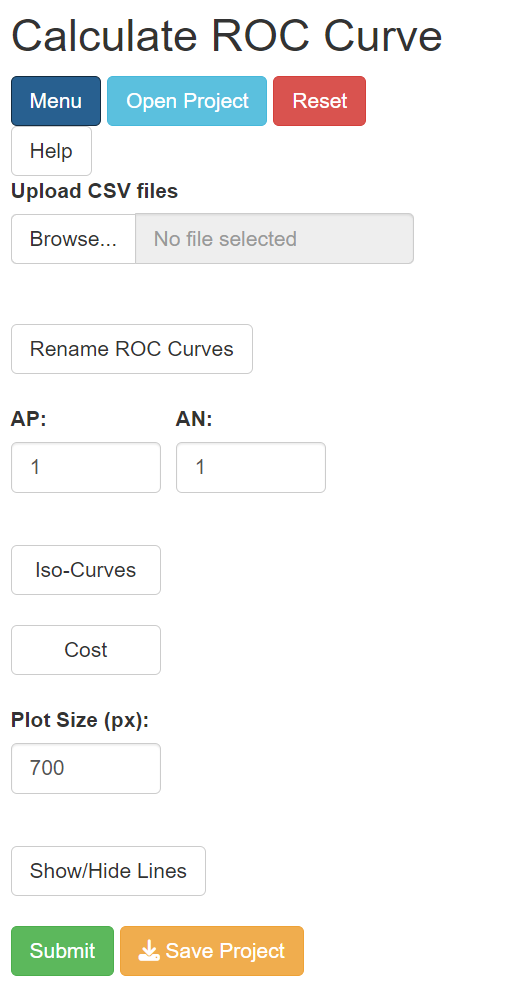
\includegraphics[width=0.7\linewidth]{Figures/screenMenu.png}
	 \end{figure}
	 
	 \subsubsection{Loading a ROC Curve}
	 The user can upload a file that represents a ROC curve. In this version, the file must be a .csv file containing at least two columns: one for the FPR values of all the points of the ROC curve, and one for the TPR values. The two columns must be named \textbf{FPR} and \textbf{TPR}, respectively.
	 
	 The .csv can have two optional columns as well. 
	 
	 One must be named \textbf{Thresholds}, and contains the threshold used to obtain a specific point of the ROC curve.
	 
	 To upload multiple curves with one file, the user must add a \textbf{Name} column. Each curve will have a different name, which has to be assigned to each point of the ROC curve. This column can be used for just one curve as well. 
	 If no Name column is present, the tool will assign the name of the file to the curve. It is not possible to load multiple curves with one file without a Name column.
	 
	 Table~\ref{tab:csvExample} shows an example of .csv, and Figure~\ref{fig:examplePlots} is the resulting plot. 
	 
	 \begin{table}[h!]
	 	\centering
	 	\label{tab:csvExample}
	 	\caption{Example of .csv file with multiple curve.}
	 	\begin{tabular}{ccl}
	 		FPR & TPR & Name         \\
	 		0   & 0   & Curve Test 1 \\
	 		0.2 & 0.3 & Curve Test 1 \\
	 		0.7 & 0.9 & Curve Test 1 \\
	 		1   & 1   & Curve Test 1 \\
	 		0   & 0   & Curve Test 2 \\
	 		0.4 & 0.4 & Curve Test 2 \\
	 		0.6 & 1   & Curve Test 2 \\
	 		1   & 1   & Curve Test 2
	 	\end{tabular}
	 \end{table}
	 
	 \begin{figure}[h!]
	 	\centering
	 	\caption{Resulting plot of the .csv file in Table~\ref{tab:csvExample}.}
	 	\label{fig:examplePlots}
	 	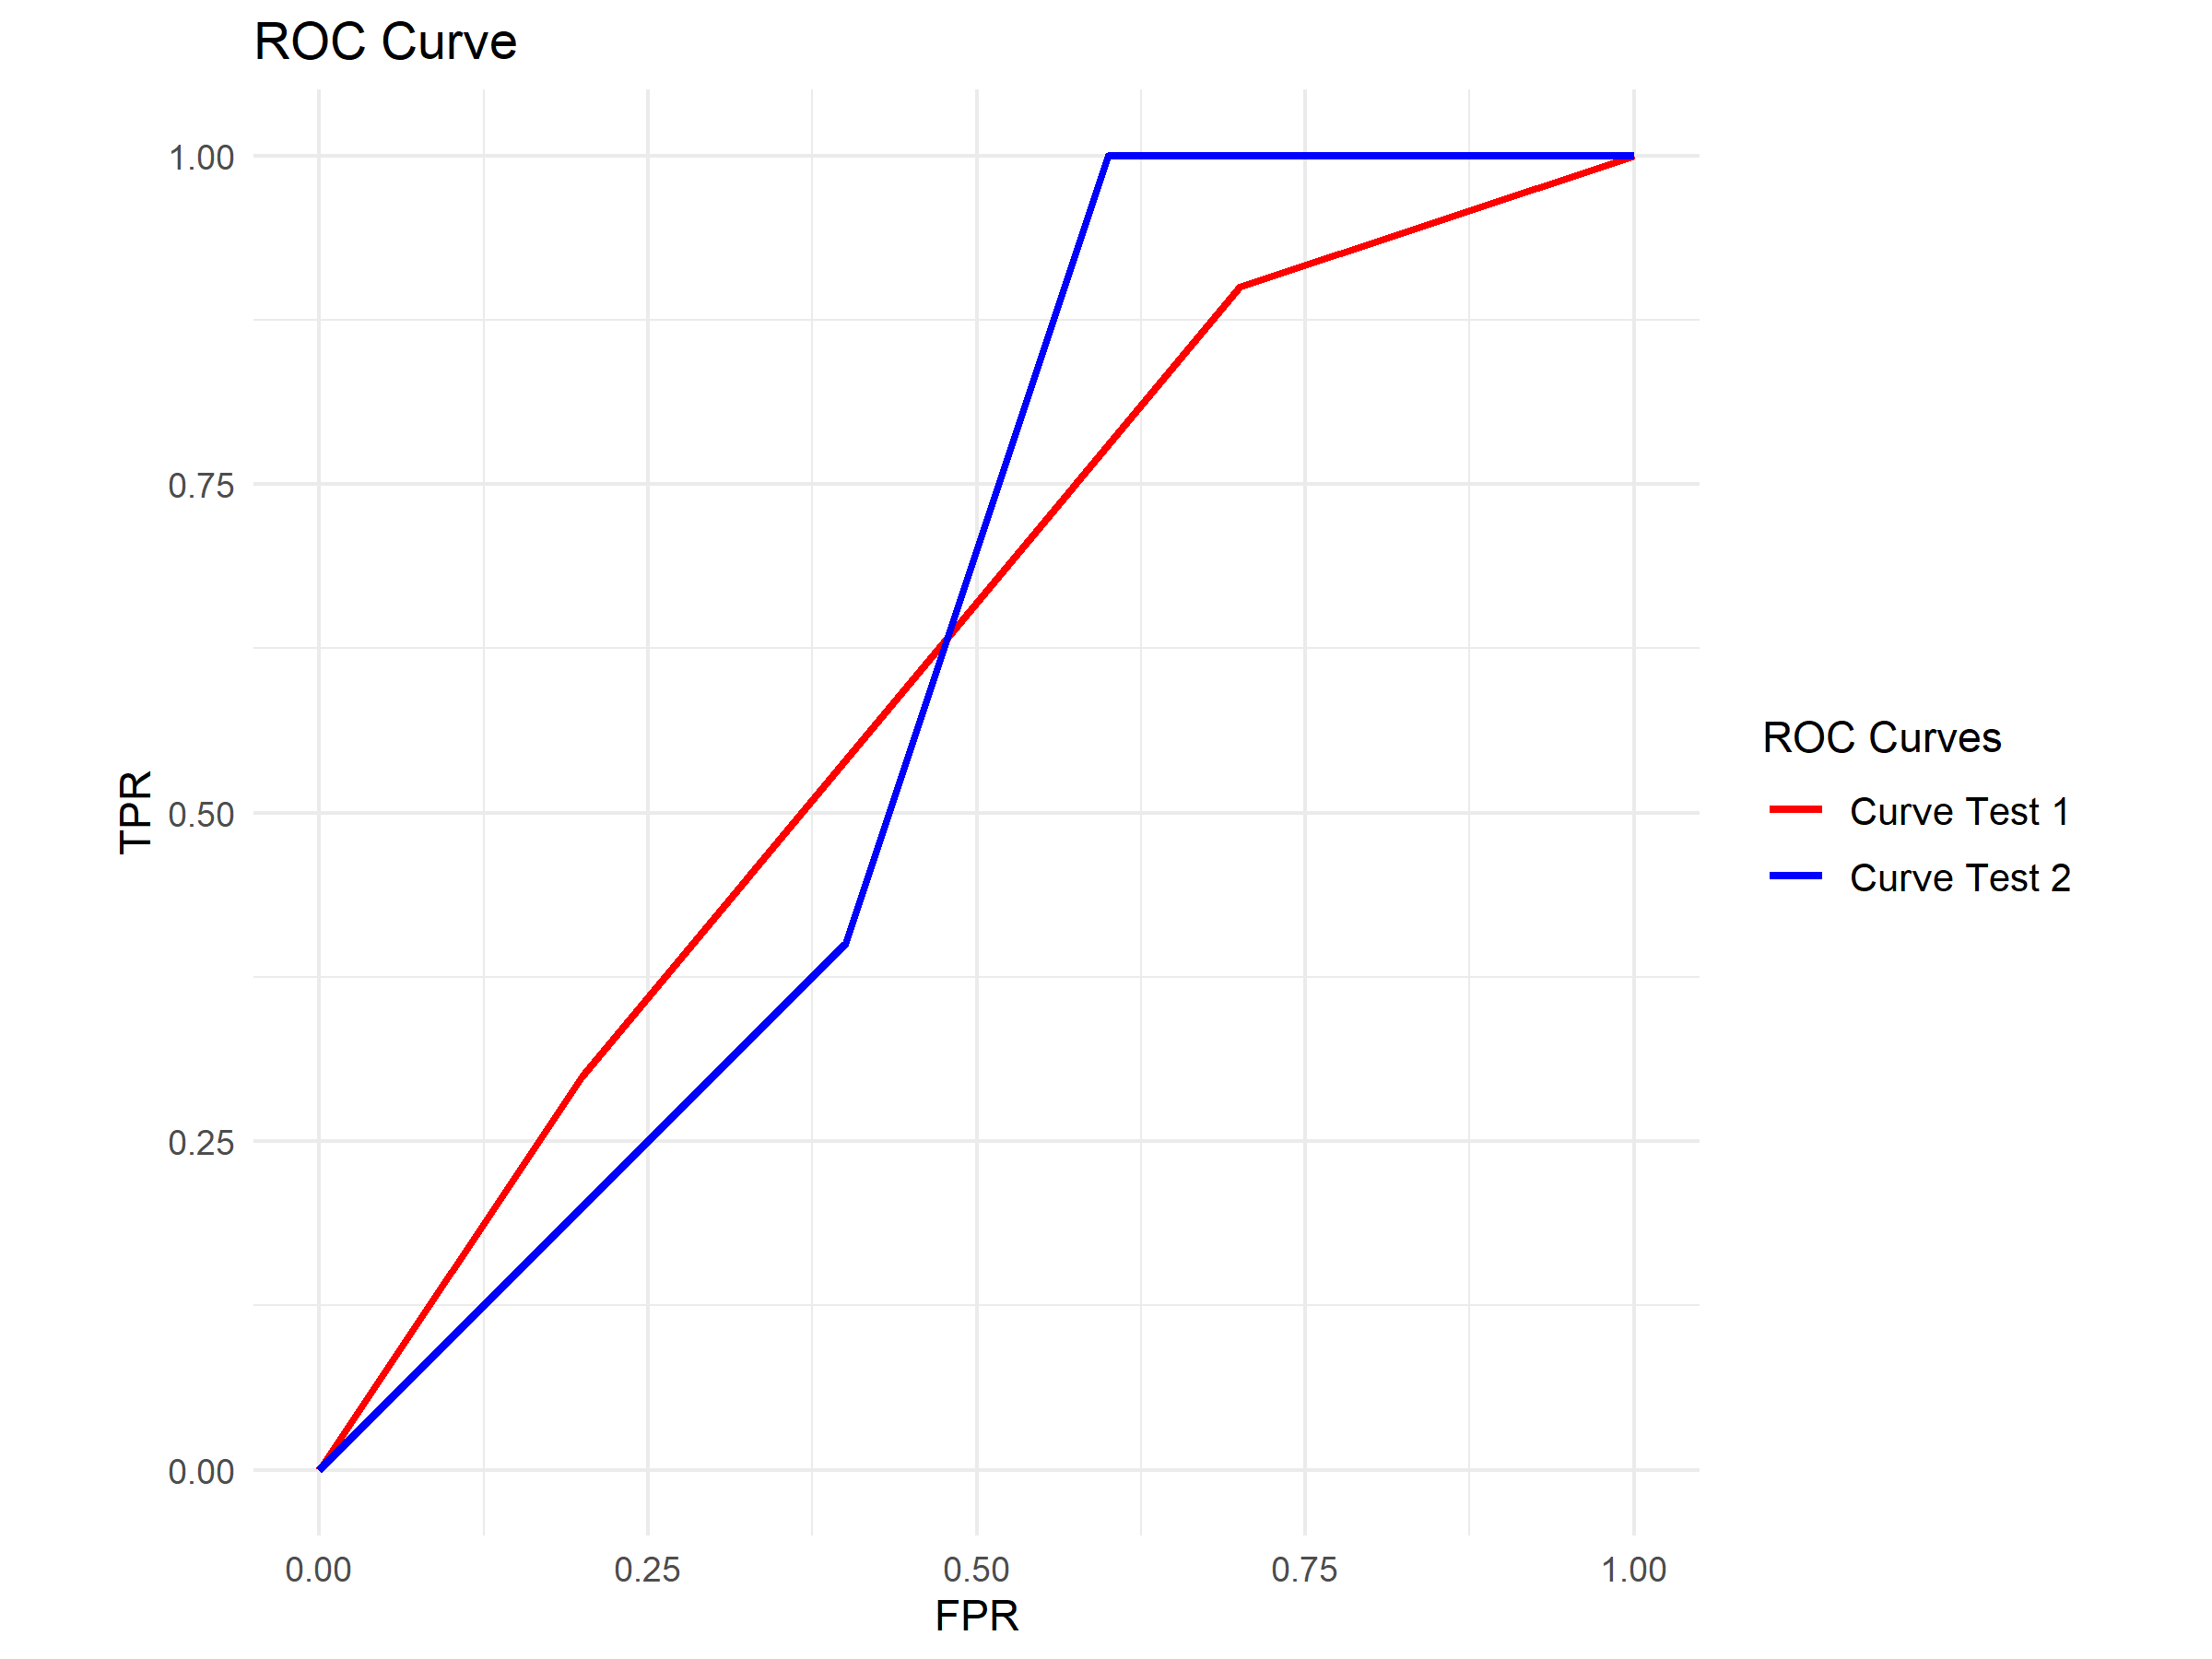
\includegraphics[width=1\linewidth]{Figures/roc_plot_1.png}
	 \end{figure}
	 
	 Before generating the plot, the user needs to set the AP and AN values. These values represent the number of positive (Actual Positives, AP) and negative (Actual Negatives, AN) elements in the test dataset used to test the model and generate the ROC curve. 
	 This value can be changed later, but all ROC curves share the same values. This is because, in order to properly confront multiple ROC curves, all curves should be generated from the same test dataset.
	 
	 The user can then select the size of the plot.
	 
	 To plot the curve, the user needs to press the "Submit" button.
	 
	 The result is presented in Figure~\ref{fig:submitresult}. By default, the plot shows the ROC curve, the boundaries of the RoI (That are, the lines $FPR=\rho$ and $TPR=\rho$, where $\rho = AP/(AP+AN)$), the RoI region, and two points. These two points represent the first and last point of the ROC curve that is inside the RoI. 
	 
	 The textbox below reports some key values for each curve. When plotting just the ROC curve, the textbox shows the AUC, RRA (The area under the curve inside the RoI, divided by the area of the RoI), and the values for the two highlighted points inside the RoI. If thresholds values are provided by the presence of a Thresholds column in the .csv file of the curve, the threshold value of the two points is also reported. If none of the points of the ROC curve is inside the RoI, no point will be highlighted in the plot.
	 
	 \begin{figure}[h!]
	 	\centering
	 	\caption{An example of result after pressing "Submit".}
	 	\label{fig:submitresult}
	 	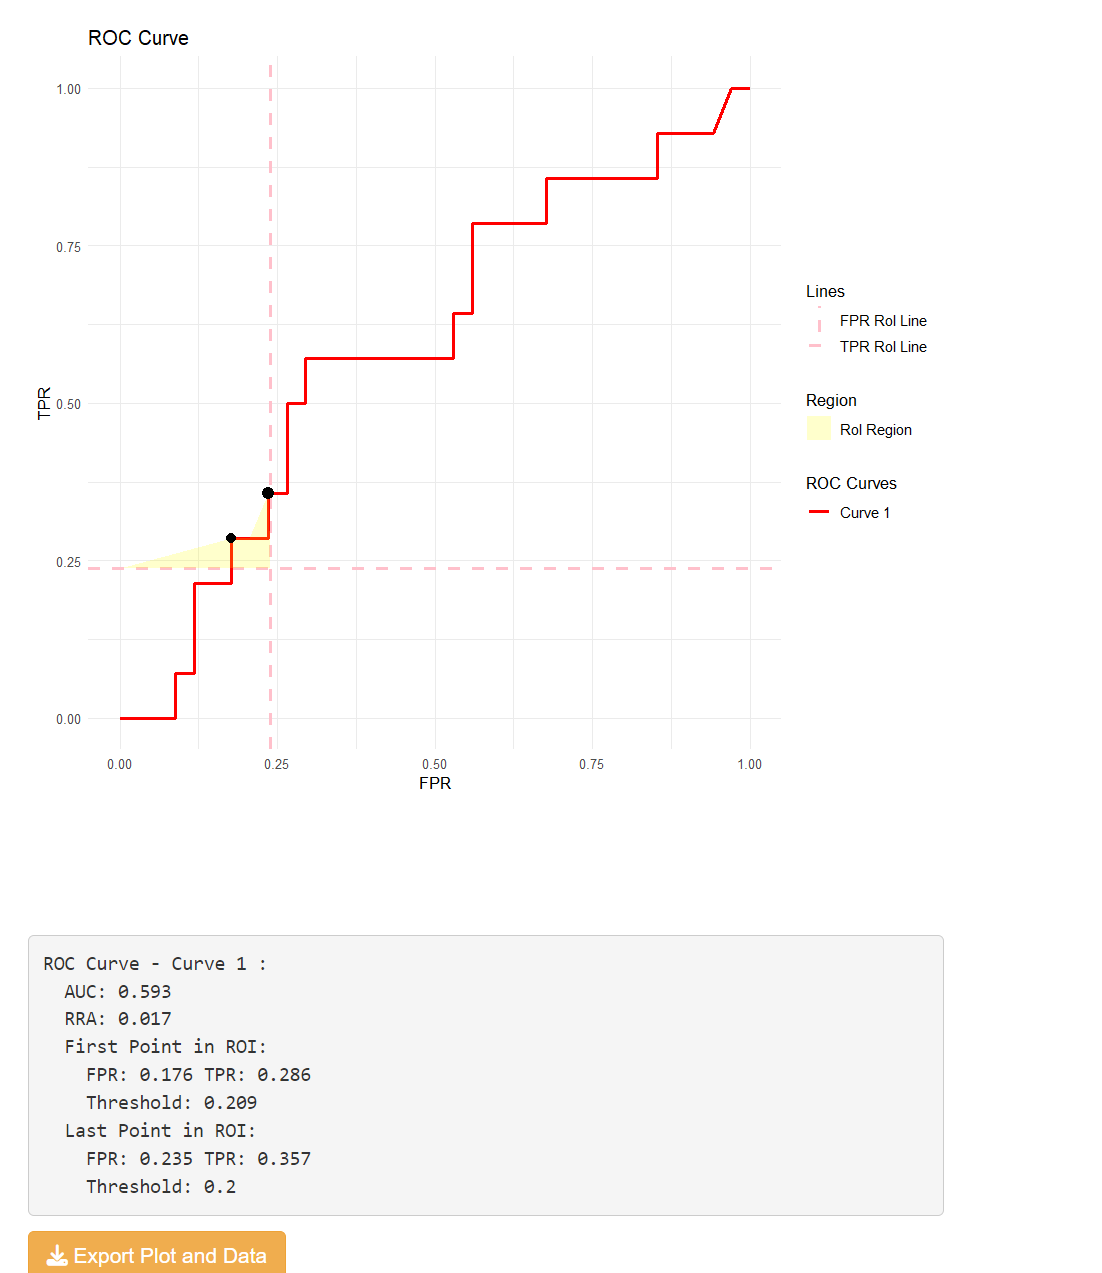
\includegraphics[width=1\linewidth]{Figures/submit_result1.png}
	 \end{figure}
	 	 
	 \subsubsection{Doing More Advanced Analysis With Iso-PM ROC Curves} 	 
	 \toolnameITB is not just a simple ROC curve plotter. The main feature of the tool is to provide an easy and straight-forward way to plot and study iso-PM ROC curves.
	 
	 By pressing the "Iso-Curves" button, the relative sub-menu becomes visible (Figure~\ref{fig:isoSubMenu}). This version of the tool is able to generate a family of iso-PM curves, from the minimum to the maximum values with a step that can be set up in the "Interval Iso-Curve:" textbox. This family of curves allows the user to give a quick glance at which PM interval a specific point of the ROC curve resides in, as seen in Figure~\ref{fig:isoFamPlot}. To choose which metrics to plot, the user can select a metric from the ones available (see Section~\ref{sec:pmSection}) in the "Iso-Curve Metric:" textbox. It is also possible to plot iso-PM curves for multiple metrics if needed. In Figure~\ref{fig:isoFamPlot} the iso-MCC curves with a interval of 0.2 have been plotted.
	 
	 \begin{figure}[h!]
	 	\centering
	 	\caption{Sub-menu that allows the user to create iso-PM curves.}
	 	\label{fig:isoSubMenu}
	 	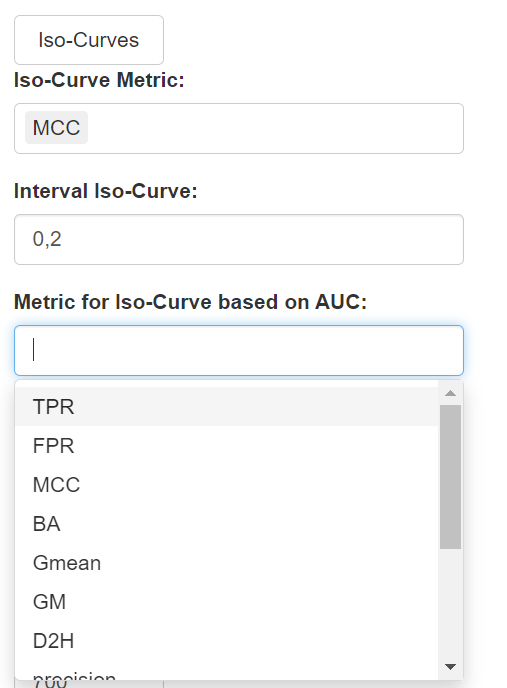
\includegraphics[width=1\linewidth]{Figures/iso_curves_submenu.png}
	 \end{figure}
	 
	 \begin{figure}[h!]
	 	\centering
	 	\caption{Plot showing the curve in Figure~\ref{fig:submitresult} with a family of iso-MCC curves with an interval of 0.2.}
	 	\label{fig:isoFamPlot}
	 	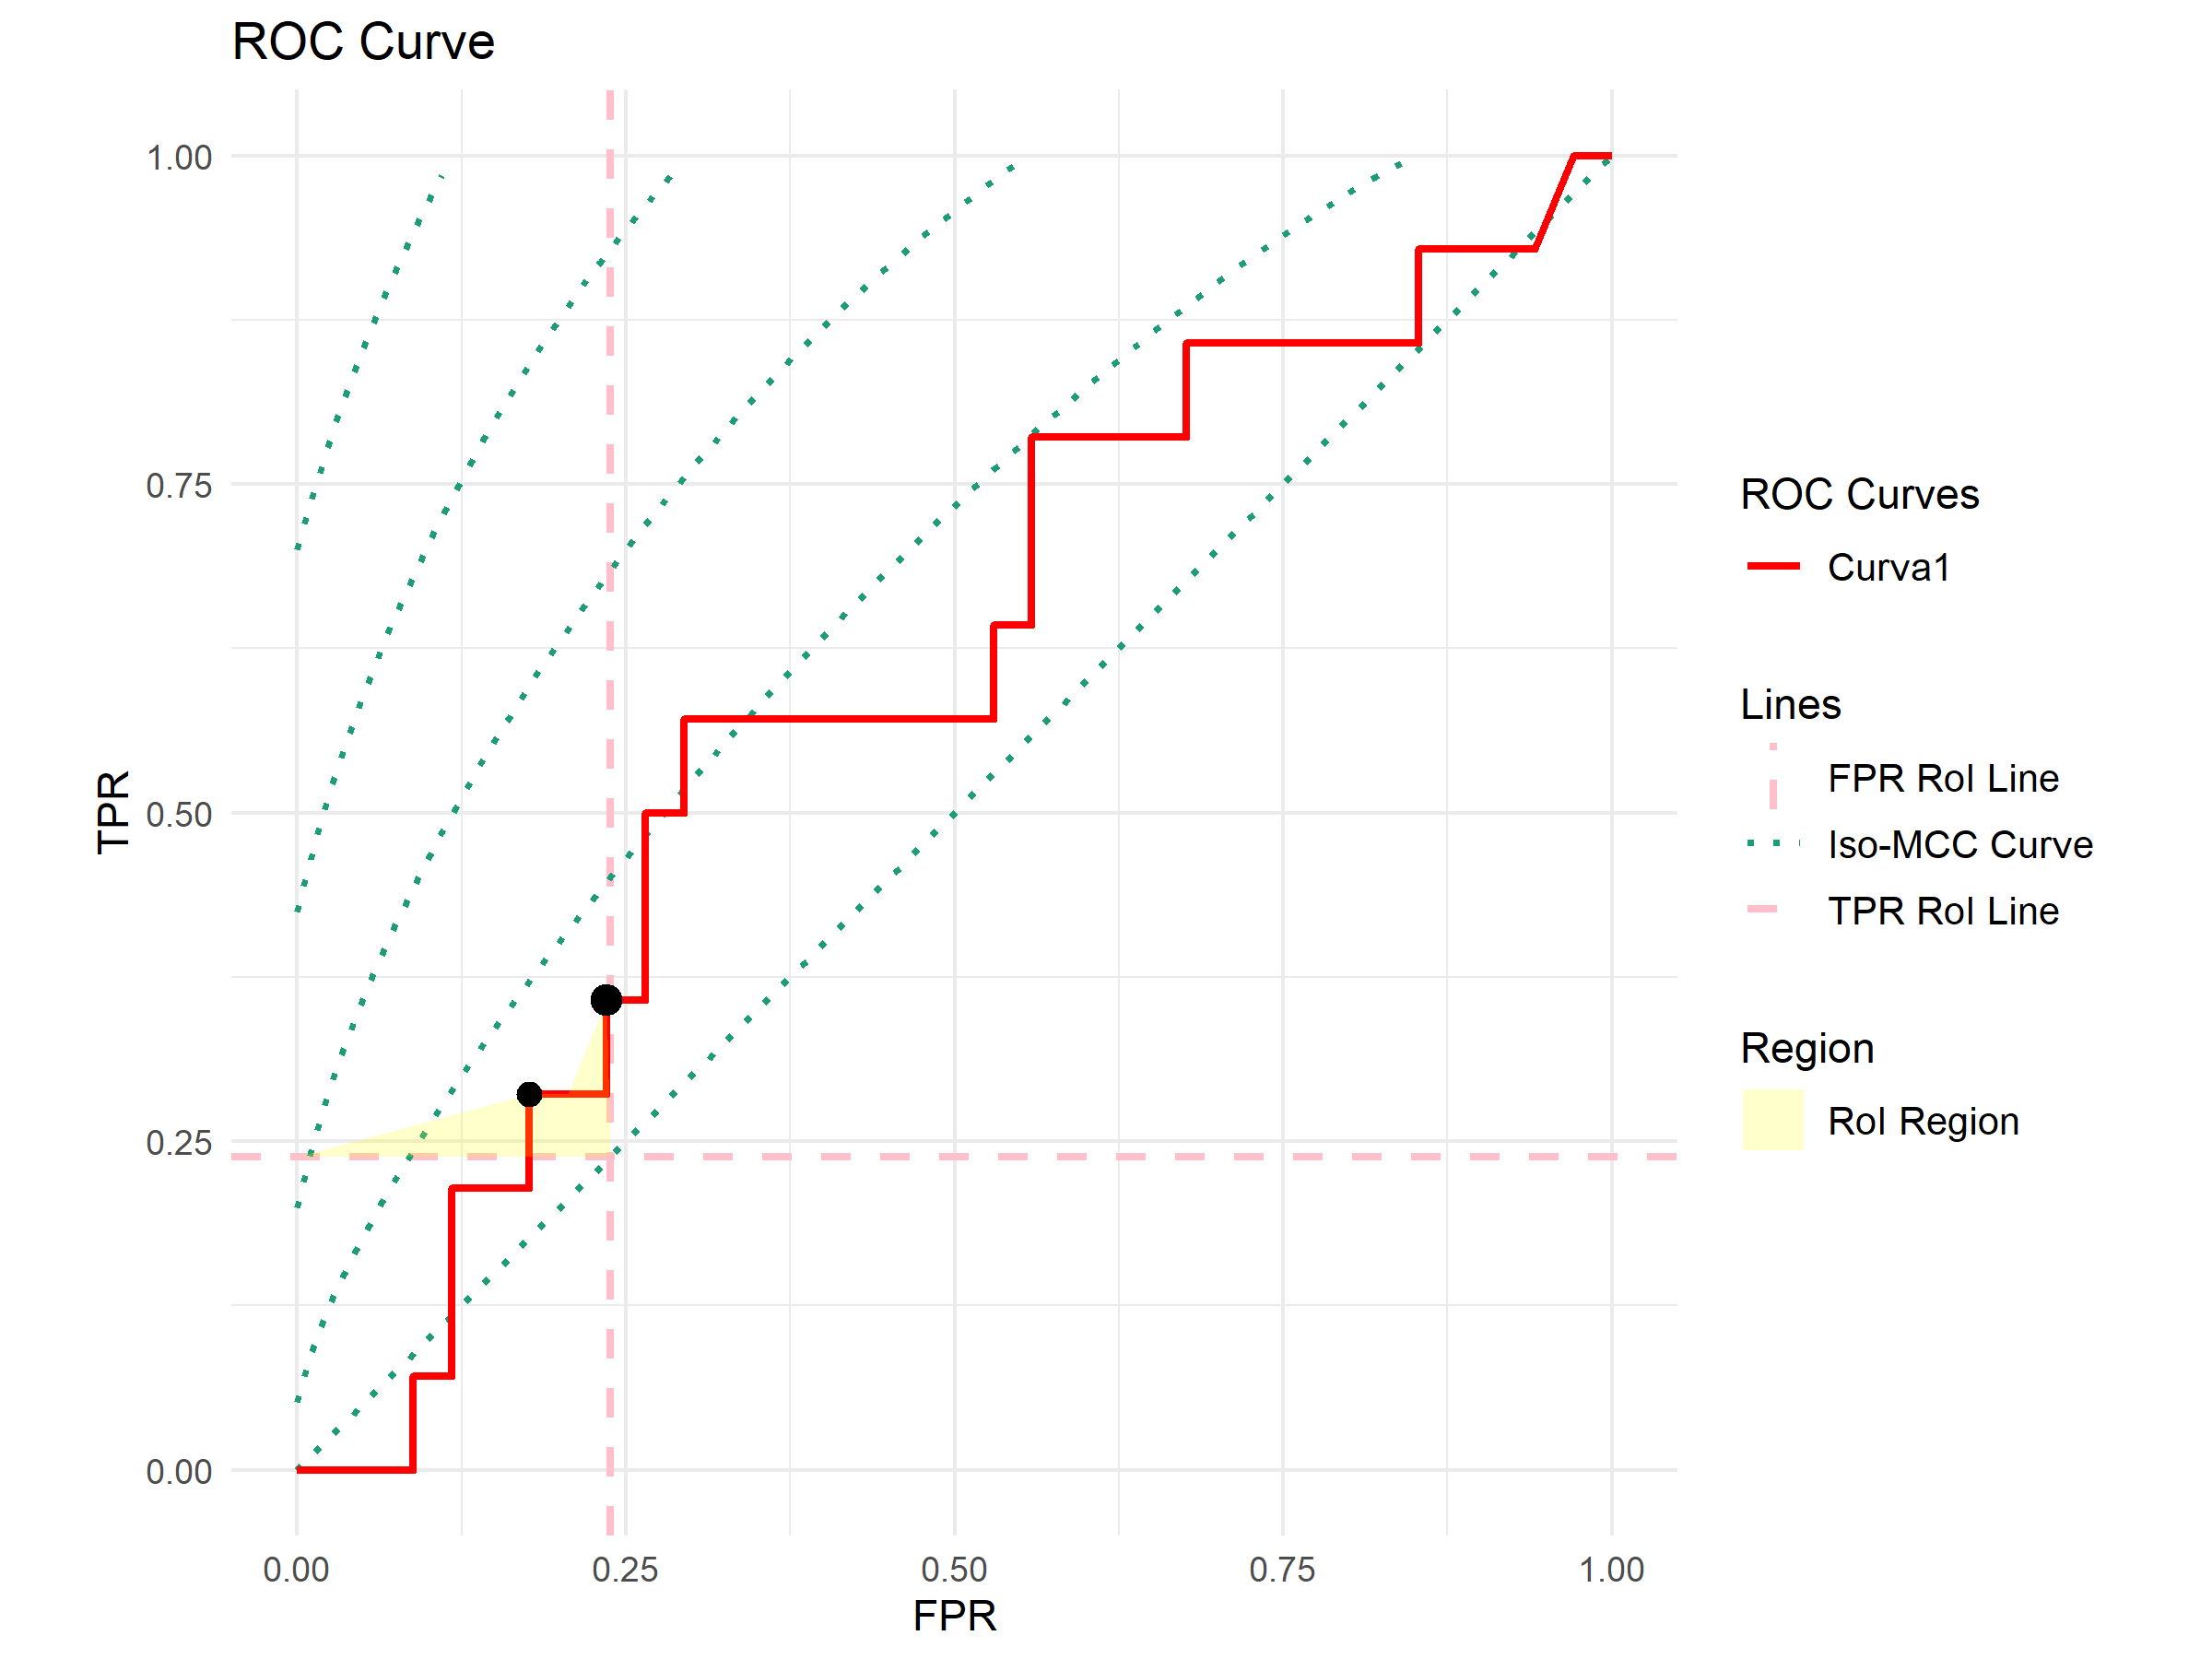
\includegraphics[width=1\linewidth]{Figures/plot_family_iso.png}
	 \end{figure}
	 
	 \subsubsection{Specific Iso-PM Curves with the same AUC and RRA Values}
	 The tools also allows to generate iso-PM curves that have the same AUC and RRA values. This way, the user can obtain a "general" PM value for the entire ROC curve. To do so, the user needs to select the PMs in the "Metric for Iso-Curve based on AUC:" and "Metric for Iso-Curve based on RRA:" (Figure~\ref{fig:isoSubMenu}) textboxes for AUC and RRA, respectively.
	 
	 The tool will compute the PM value that generates the iso-PM curve with the same AUC/RRA as the original ROC curves. The resulting iso-PM curves are plotted, and the PM values for each curves are printed in the textbox below the plot. An example is represented in Figure~\ref{fig:isocurveAUC}.
	 
	 \begin{figure}[h!]
	 	\centering
	 	\caption{Iso-MCC curves added for two ROC curves.}
	 	\label{fig:isocurveAUC}
	 	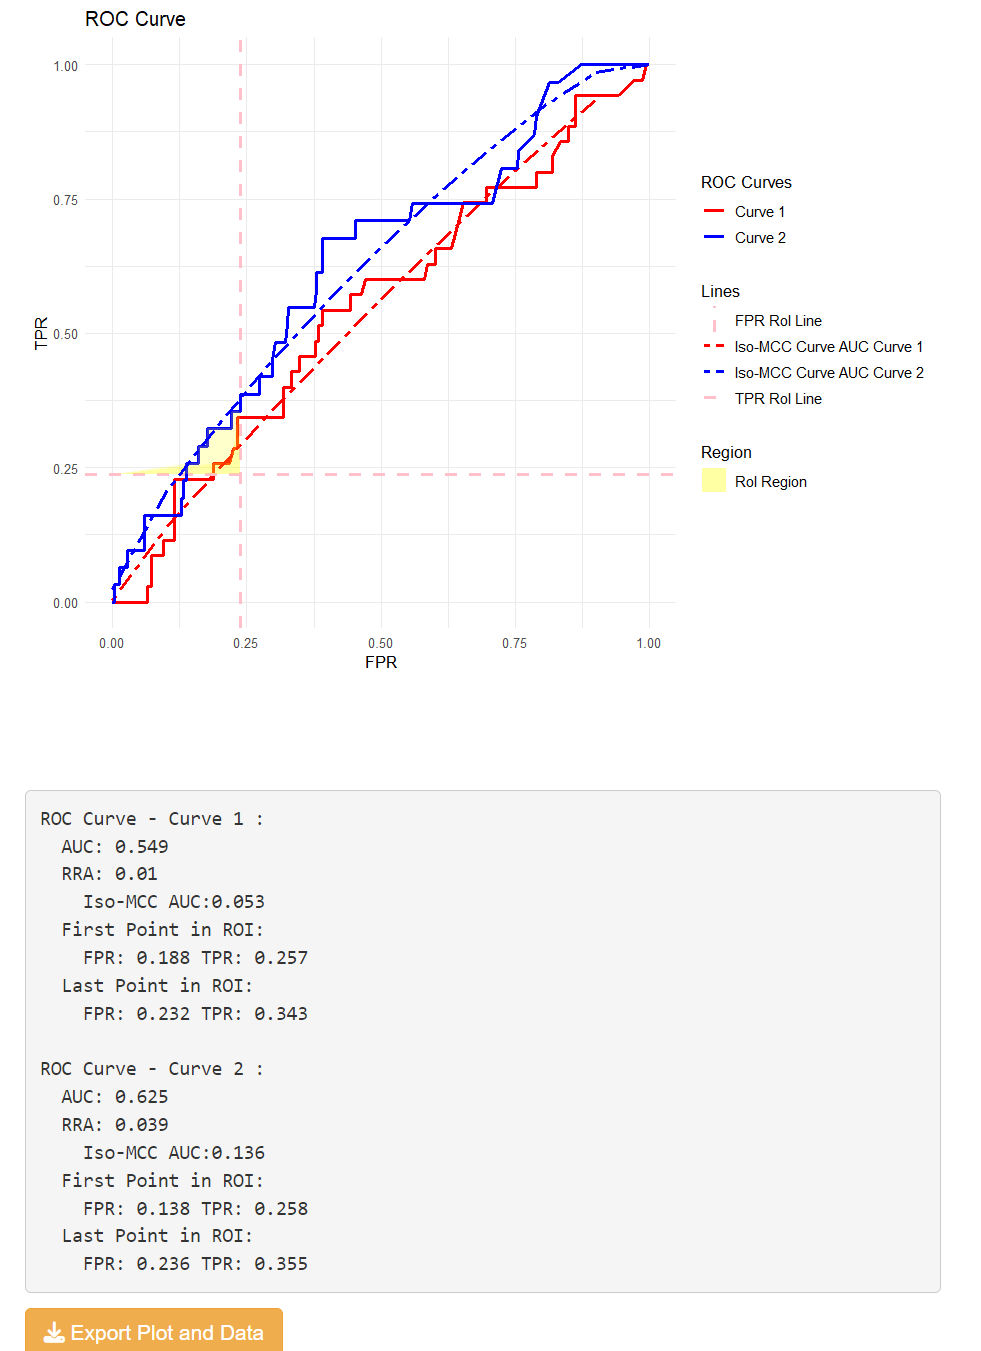
\includegraphics[width=1\linewidth]{Figures/iso_cost_result_plot_print.png}
	 \end{figure}
	  
	 \subsubsection{Iso-Cost ROC Curves}
	 To build families of iso-cost curves, the user needs to use a different sub-menu, which is shown by pressing the "Cost" button in the Menu, shown in Figure~\ref{fig:isocostSubMenu}. Unlike other iso-PM curves, the user needs to set the unitary costs for False Positives and Negatives (cFP and cFN). Aside from that, it works exactly like the generation of other iso-PM curves.
	 
	 \begin{figure}[h!]
	 	\centering
	 	\caption{Iso-cost sub-menu.}
	 	\label{fig:isocostSubMenu}
	 	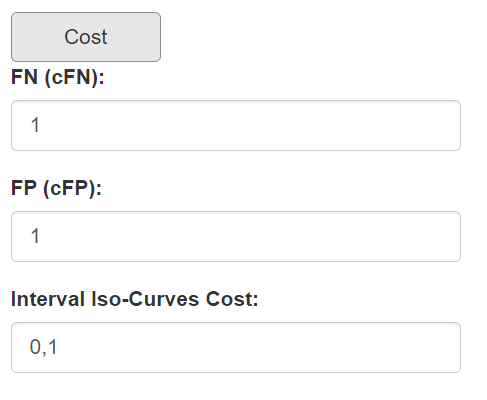
\includegraphics[width=1\linewidth]{Figures/iso_cost_submenu.png}
	 \end{figure}
	
	 \subsubsection{Updating the Plot, Hide Elements, and Rename the Curve}
	 After pressing the "Submit" button, it is possible to update the values in the Menu. When values are changed, the plot and textbox are automatically updated. There is no need to press "Submit" again, unless the user wants to add a new curve to the plot.
	 
	 By pressing the "Rename ROC Curves" button, it is possible to change the name assigned to each curve. To apply the changes, the user needs to press the "Save Changes" button.
	 
	 By pressing the "Show/Hide Lines" button, a list of checkboxes is shown. These checkboxes indicate what to plot and what to hide. This allows users to load many ROC curves, generating multiple iso-PM curves, and making multiple analysis, without having to reset, and without making the plot completely unreadable. 
	 
	 The names are self-explanatory. 
	 
	 \subsection{Save and Load a Project} \label{ssec:oploconfigs}
	 It is possible to save progress to load them at a later time, or to share them with other users.
	 
	 To do so, the user needs to press the "Save Project" button. Now, the user can choose where to save the project and rename it. The project is saved in a .rds file.
	 
	 To load a project, the user needs to press the "Open Project" button, next to the "Menu" button and select the .rds file. The tool will update all values in the menu's fields, generate the plot, and print the results.
	 
	 \section{Exporting the Results}
	 If the user wants to export the plot and results obtained, they can press the "Export Plot and Data" button below the textbox (Figure~\ref{fig:submitresult}). The user then needs to choose a location a rename the file.
	 
	 The exported file is a compressed .zip folder. This folder contains two files: \texttt{roc\char`_data.xhtml} and \texttt{roc\char`_plot.png}. By extracting the folder, it is possible to open the .xhtml file to see all the produced data and the plot. The .png file only contains the plot.
	 
	 \begin{figure}[h!]
	 	\centering
	 	\caption{The resulting .xhtml file of an exported project. The plot is slightly cut in the Figure to make it more readable in this Documentation.}
	 	\label{fig:exportResult}
	 	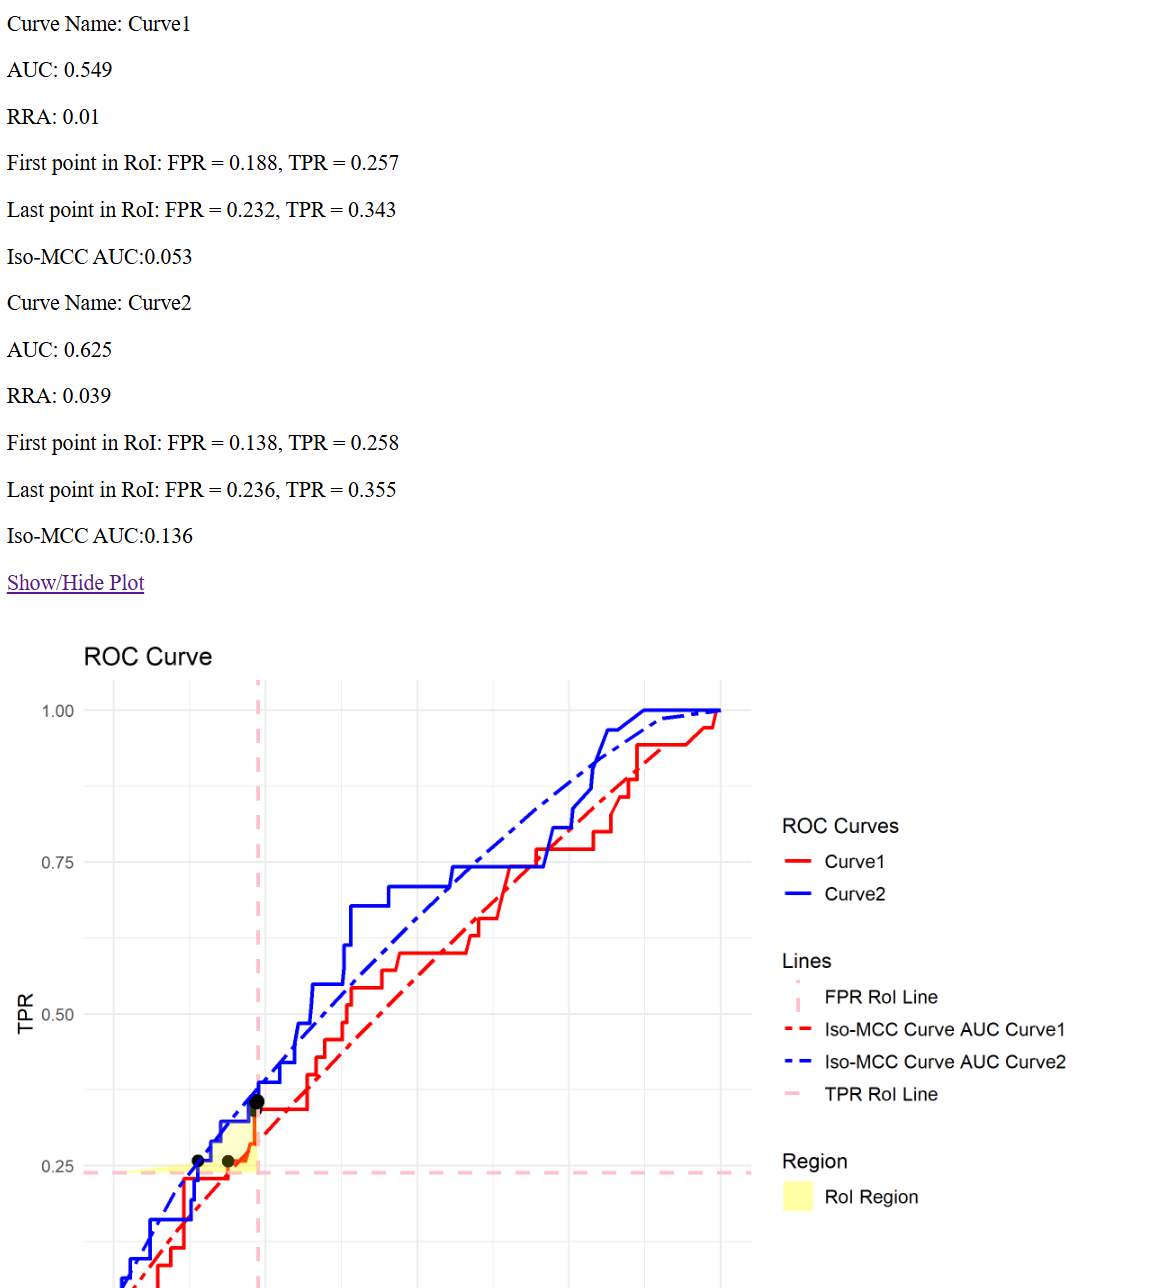
\includegraphics[width=1\linewidth]{Figures/export_result.png}
	 \end{figure}
	 
	 \bibliographystyle{plain} 
	 \bibliography{refs}
	 
\end{document}

